\documentclass[12pt]{article}
\usepackage[top=1in, bottom=1in, left=1in, right=1in]{geometry}
\usepackage[justification=centering]{caption}
\usepackage{graphicx}
\usepackage{listings}

\begin{document}
\title{Microprocessor Systems \\ Lab 1: IDE \&\ ANSI Display}
\author{Nick Choi \and Samuel Deslandes}
\date{}
\maketitle

\section{Introduction}
The overall goal of this lab is to become familiar with utilizing the registers on the 8051 as well as performing fundamental I/O operations with it. This lab also served as an introduction to the VT100 Terminal and the utilization of he ANSI escape sequences it features. 

This lab was divided into 3 parts. The first was an exercise in basic terminal I/O in which a C program was written to await a user keystroke and, if printable, output it on the terminal display. The second part was an enhancement of the first part but heavy usage of the ANSI escape codes to format text on the display. The ANSI escape codes are special sequences beginning with \textless ESC\textgreater (\textbackslash033 in octal or \$1B in hex) which modify terminal behavior, adding features such as underlined text, background/foreground color changes, changing the cursor position, selectable scrolling, etc... The third part of the lab involved configuring ports on the 8051 to be either inputs or outputs. In this part of the lab hardware connected to the input port could be used to change the state of hardware connected to the output ports of the 8051. 

\section{Methods}
\subsection{Software}
The code for parts 1, 2 and 3 can be found in Appendix A, B and C respectively. All code was uploaded and run on the 8051 through the programming/debugging USB port. 	

In the first section of the lab, a C program was written so that user input from a keyboard could be displayed in the ANSI terminal. The 8051 determined which keyboard character was pressed by utilizing the ``getchar()'' and ``putchar()'' functions defined in the ``putget.h'' header file. It should be noted that the ``getchar()" function was modified from the original header file to not echo captured keystrokes. Whenever a printable character was input, it was printed to the terminal display with the following message: "The keyboard character is *."  Unprintable characters were not displayed and the program would run in an infinite loop unless the \textless ESC\textgreater key was pressed. Pressing the \textless ESC\textgreater key both restarted the C program and cleared the terminal. In order to determine whether the input was printable or not, the captured character's ASCII was compared with the printable characters on the ASCII table, which range from 0x20 (space) through 0x7E (\texttt{\char`\~}).

The second part builds upon the C program written for the first so that it would incorporate escape sequences to achieve various text effects within the VT100 terminal. Table \ref{refTable} below contains all of the ANSI escape sequences used for this lab. The first modification was to change the background color to blue and the foreground color to yellow. This was done using the codes ``\textbackslash033[1;43m" and ``\textbackslash033[1;33m" respectively. The first line of text contains program termination information similar to that of part 1; It is printed on line 2 of the terminal and is horizontally centered. This can be accomplished using the escape code for changing the cursor position ``\textbackslash033[\{row\};\{col\}H". In this case 2 and 30 were used for the row and column respectively.
As was done in part 1, the keyboard response must also be displayed, this time on line 6 with the keyed in character printed in white. The same code above was used to jump the cursor to line 6, and ``\textbackslash033[1;37m" is used to change the text's color to white. If the keyed in character is not printable, the message "The keyboard character \$XX is \underline{'not printable'}." should appear starting halfway down the terminal (line 12 in our case) and work its way down the screen. This text should be blinking and make an audible 'BEL' noise when a non-printable character is keyed in. The terminal should be set such that only the bottom half of the screen scrolls. Although the escape code to change the position of the cursor could be used accomplish this, the codes to save and restore the cursors position were used instead so that we would not have to directly keep track of what line to jump to. In order to do this we had it so that before a non-printable is even keyed in the position of the next error message was already stored so that when it came time to print the error message all that had to be done was restore the cursor position, print the error message ending it with the ASCII newline escape sequence ('\textbackslash n'), then save this position before returning to waiting for user input. The ANSI codes for saving and restoring the cursor's position are ``\textbackslash033[s" and ``\textbackslash033[u" respectively. To get the audible feedback portion the ASCII escape sequence '\textbackslash a' was used. When writing the code block pertaining to printing the error message, it is important to remember to turn off the underscore and blinking once the desired text with these effects has been printed.

\begin{table}[h]
	\centering
	\begin{tabular}{|l|l|}
		\hline
		\textbackslash033[2J & Clear screen and return cursor to home \\ \hline
		\textbackslash033[1;33m & Set text color to yellow \\ \hline
		\textbackslash033[1;43m & Set background color to blue \\ \hline
		\textbackslash033[1;37m & Set text color to white\\ \hline
		\textbackslash033[{row};{col}H & Move cursor position to (\{row\},\{col\})\\ \hline
		\textbackslash033[{start};{stop}r & Set scroll area from \{start\} to \{stop\}\\ \hline
		\textbackslash033[s & Save cursor position\\ \hline
		\textbackslash033[u & Restore cursor position\\ \hline
		\textbackslash033[5m & Turn blinking text on\\ \hline
		\textbackslash033[25m & Turn blinking text off\\ \hline
		\textbackslash033[4m & Underline text\\ \hline
		\textbackslash033[24m & Turn underline text off\\ \hline		
		\hline
	\end{tabular}
	\caption{Quick reference table of ANSI escape sequences}
	\label{refTable}
\end{table}

Part 3 took the code in a very different direction and focused more on the hardware than the software. In terms of software, all of port 1 had to be configured to be in open-drain mode (input), and all of port 2 to push-pull mode (output). This was done by setting all of the bits of the P1MDOUT special function register (SFR) low, and all of those of P2MDOUT high. This should be done in the 'PORT\_INIT()' function. In the main function, all that had to be done was read the value of port 1 into port 2. This could be done using the P1 and P2 port SFRs. 

\subsection{Hardware}

Parts 1 and 2 of this lab did not require any hardware other than a serial-to-USB adapter in order to interface with the terminal.

In the third section of the lab, the pins on port 1 were connected to the input device, the potentiometer module, and pins on port 2 were connected to the output device, the LED module. Since there were only 4 potentiometers on the potentiometer module only the first 4 pins on each port were used (P1.0 - P1.3 and P2.0 - P2.3). These corresponded to pins 12, 13, 10, and 11 on the EVB for port 1, and 29, 30, 27, and 28 for port 2. A circuit diagram can be seen in figure \ref{schematic} below.

The input pins of the module have inverters incorporated into them so that whenever a logic high is applied to an input pin, the signal is changed to be a logic low. This inversion allows the LED to illuminate because there will be a voltage difference across the anode and cathode of the LED. If a logic low is applied to the input pin, the signal is changed to be a logic high. This removes the voltage difference between the anode and cathode of the LED and thus prevents the LED from lighting up. 

\begin{figure}[h]
	%\centering
	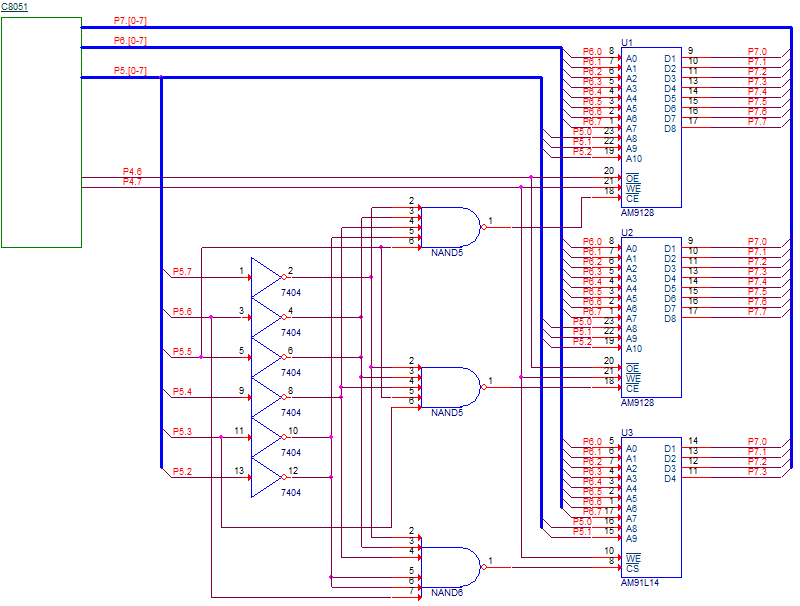
\includegraphics{schematic.png}
	\caption{Circuit schematic for part 3}
	\label{schematic}
\end{figure} 
 
\section{Results}

By completing section one of the lab, a functioning C program was produced which read keyboard input and displayed it in an ANSI terminal. After completing section two, an improved version of the program from section one was produced. This version reacted to user input and manipulated the output of the ANSI terminal in several ways. The final deliverable was an LED module which was controlled by a potentiometer module. 

\section{Conclusion}

\section{Appendices}

\subsection{Modified putget.h}
	\lstinputlisting{putget.h}
\subsection{Part 1}
	
\subsection{Part 2}
	\lstinputlisting{part1.c}
\subsection{Part 3}
	\lstinputlisting{part3.c}
	
	
\section{References} 







\end{document}